\subsection{Entrega}

\begin{table}[H]
    \centering
    \caption{Custos de execução para $N=\{12,16,24,32\}$ (média de uma única rodada).}
    \label{tab:tempo_poisson}
    \begin{tabular}{c c c}
        \toprule
        $N$ & Tempo de solução (s) & Tempo de interpolação (s) \\
        \midrule
        12 & 1.3153 & 0.3482 \\
        16 & 0.0011 & 0.0024 \\
        24 & 0.0059 & 0.0024 \\
        32 & 0.0279 & 0.0024 \\
        \bottomrule
    \end{tabular}
\end{table}

\begin{table}[H]
    \centering
    \caption{Erros máximos entre discretizações consecutivas na malha fina.}
    \label{tab:erro_poisson}
    \begin{tabular}{c c}
        \toprule
        Par de discretizações & $\max | \Delta u |$ \\
        \midrule
        $12 \leftrightarrow 16$ & $6.0753 \times 10^{-2}$ \\
        $16 \leftrightarrow 24$ & $3.5876 \times 10^{-2}$ \\
        $24 \leftrightarrow 32$ & $2.0015 \times 10^{-2}$ \\
        \bottomrule
    \end{tabular}
\end{table}

\begin{figure}[H]
    \centering
    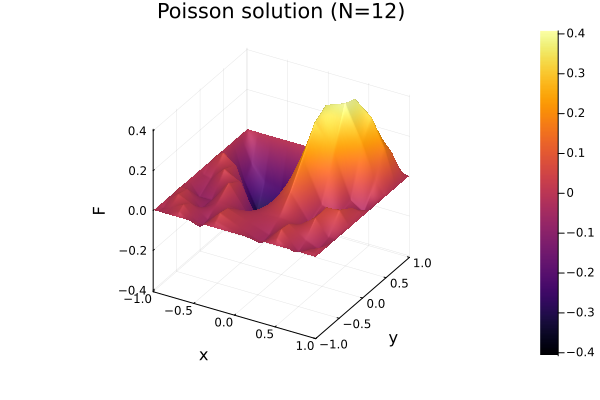
\includegraphics[width=0.48\textwidth]{code/../figures/surface_N12.png}
    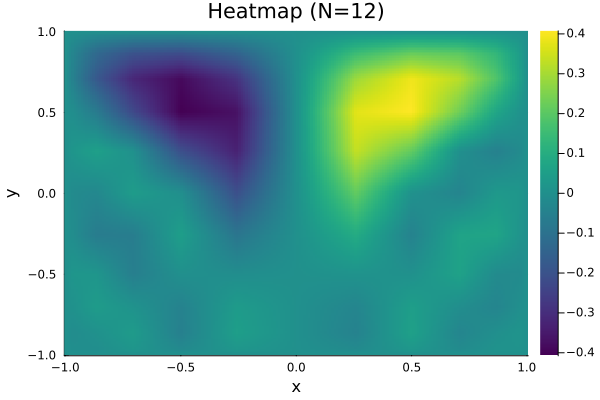
\includegraphics[width=0.48\textwidth]{code/../figures/heatmap_N12.png}\\[4pt]
    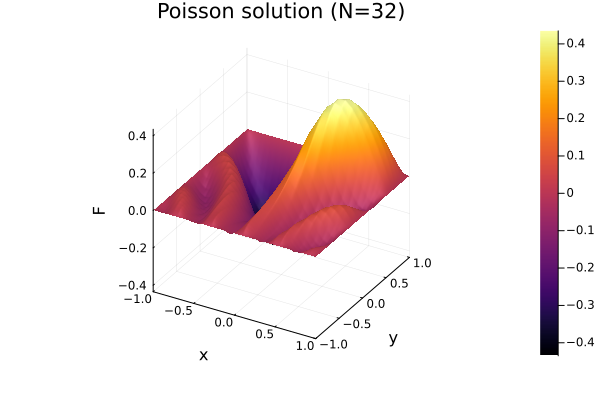
\includegraphics[width=0.48\textwidth]{code/../figures/surface_N32.png}
    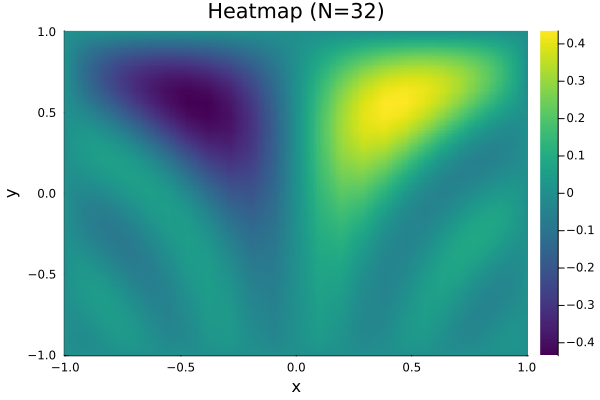
\includegraphics[width=0.48\textwidth]{code/../figures/heatmap_N32.png}
    \caption{Superfícies e mapas de calor para $N=12$ (linha superior) e $N=32$ (linha inferior). Os demais gráficos seguem o mesmo padrão no diretório \texttt{\_hw9/figures}.}
    \label{fig:poisson_surfaces}
\end{figure}

\paragraph{Implementação em Julia} O pacote \texttt{SpectralTools} encapsula utilidades genéricas (vectorização, matrizes de diferenciação e solver de Poisson 2D) com testes automatizados. O script \texttt{solve\_poisson\_hw9.jl} reutiliza essas rotinas, executa várias ordens de Chebyshev--Lobatto, interpola em uma malha $200\times200$ usando \texttt{Interpolations.jl} e gera figuras com \texttt{Plots.jl}. Toda a lógica está modularizada para permitir reaproveitamento em outras tarefas espectrais.

\paragraph{Discussão das discretizações} A Tabela~\ref{tab:erro_poisson} mostra redução monotônica do erro ao refinar $N$, evidenciando convergência espectral suave para a solução senoidal. A queda de $6.1\times10^{-2}$ para $2.0\times10^{-2}$ entre as discretizações extremas confirma a melhora qualitativa observada nas Figuras~\ref{fig:poisson_surfaces}, onde a geometria da solução fica mais definida e a amplitude é melhor capturada.

\paragraph{Dificuldades} A principal dificuldade prática foi preparar o ambiente gráfico em modo \emph{headless}. Foi necessário configurar \texttt{ENV["GKSwstype"]="100"} para que o backend GR gerasse PNGs sem display. Além disso, a comparação entre malhas exigiu interpolar soluções com malhas distintas, motivando o uso explícito do módulo \texttt{Interpolations}.

\subsection{Implementação Espectral em Julia}

O trecho a seguir resume o solver reutilizável construído no pacote \texttt{SpectralTools}, responsável por aplicar o esquema de collocation de Chebyshev--Lobatto para o problema de Poisson bidimensional:

\begin{verbatim}
function poisson_chebyshev_2d(f_fun, N)
    x, D = cheb(N)
    D2 = D * D
    inner = 2:N
    D2_inner = D2[inner, inner]
    x_inner = x[inner]
    nint = length(x_inner)
    L = kron(I, D2_inner) + kron(D2_inner, I)
    xx = repeat(reshape(x_inner, 1, nint), nint, 1)
    yy = repeat(reshape(x_inner, nint, 1), 1, nint)
    rhs = vec(f_fun.(xx, yy))
    u_inner = L \ rhs
    U = zeros(nint + 2, nint + 2)
    U[inner, inner] .= unvec(u_inner, nint, nint)
    return U, x, x
end
\end{verbatim}

O procedimento segue diretamente a teoria apresentada em Trefethen (Program 16): os pontos de Chebyshev--Lobatto $x_j = \cos\big(\pi j/N\big)$ formam a malha com clustering nos contornos, e a matriz de diferenciação $D$ aproxima derivadas por interpolação polinomial global. Ao construir $D^2$ e extrair o bloco interno $D_{\text{int}}^2$ obtém-se a segunda derivada apenas nos nós interiores, o que implementa automaticamente a condição de Dirichlet homogênea ($F=0$ no contorno). O operador laplaciano discreto resulta do produto de Kronecker $L = I \otimes D_{\text{int}}^2 + D_{\text{int}}^2 \otimes I$, espelhando a separação de variáveis clássica para base de Chebyshev.

Na sequência, o script 	exttt{solve\_poisson\_hw9.jl} instancia a função fonte $f(x,y) = 10\sin(8x(y-1))$ e percorre múltiplos valores de $N$ com medições de tempo:

\begin{verbatim}
for N in (12, 16, 24, 32)
    U, x, _ = poisson_chebyshev_2d(f_fun, N)
    sorted_axis = reverse(x)
    sorted_values = reverse(reverse(U, dims = 1), dims = 2)
    interpolant = interpolate((sorted_axis, sorted_axis),
                              sorted_values, Gridded(Linear()))
    fine_vals = [interpolant(yv, xv) for yv in fine_axis, xv in fine_axis]
end
\end{verbatim}

Esse laço evidencia duas etapas teóricas: (i) a resolução espectral que fornece a solução apenas nos nós de Chebyshev e (ii) a interpolação posterior para uma malha uniforme fina, que aproxima a projeção contínua do campo resolvido. A seleção dos valores de $N$ permite observar a convergência exponencial típica dos métodos espectrais para funções suaves, como demonstrado pelas reduções de erro relatadas na Tabela~\ref{tab:erro_poisson}.
